\begin{figure}[H]
\centering
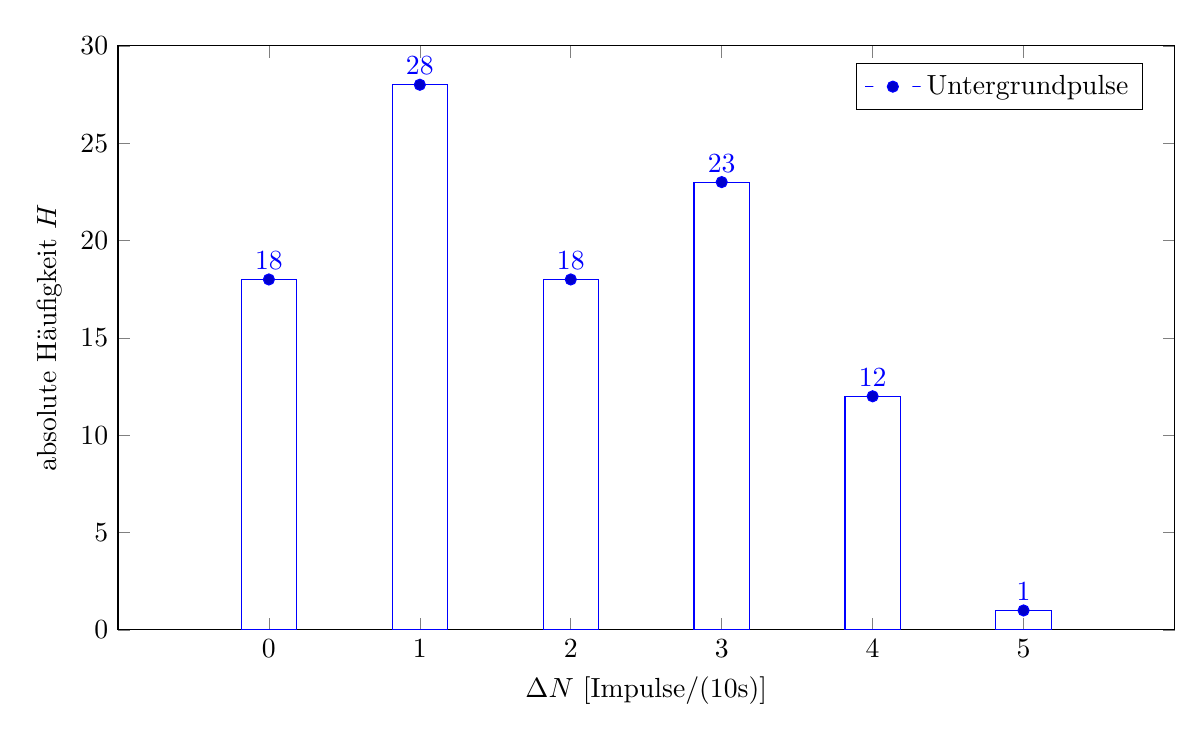
\begin{tikzpicture}
  \begin{axis}[
    width=15 cm,
    height=9 cm,
    xmin=-1, xmax=6,
    ymin=0, ymax=30,
    xlabel={$\Delta N$ [Impulse/(\SI{10}{s})]},
    ylabel={absolute Häufigkeit $H$},
    domain=-3:17,
    legend entries={Untergrundpulse},
    legend pos=north east,
		bar width=20pt,
		xtick={0,1,...,5},
		nodes near coords
  ]
  \addplot+[ybar] plot coordinates {
		(0,18)	(1,28)	(2,18)	(3,23)	(4,12)	(5,1)
		};
  \end{axis}
\end{tikzpicture}
\caption{Absolute Häufigkeitsverteilung der Untergrundpulse. Impulse innerhalb eines Intervalls von $\SI{10}{s}$ wurden zusammengefasst.}
\label{fig:untergrundabsolut}
\end{figure}
\begin{figure}[H]
\centering
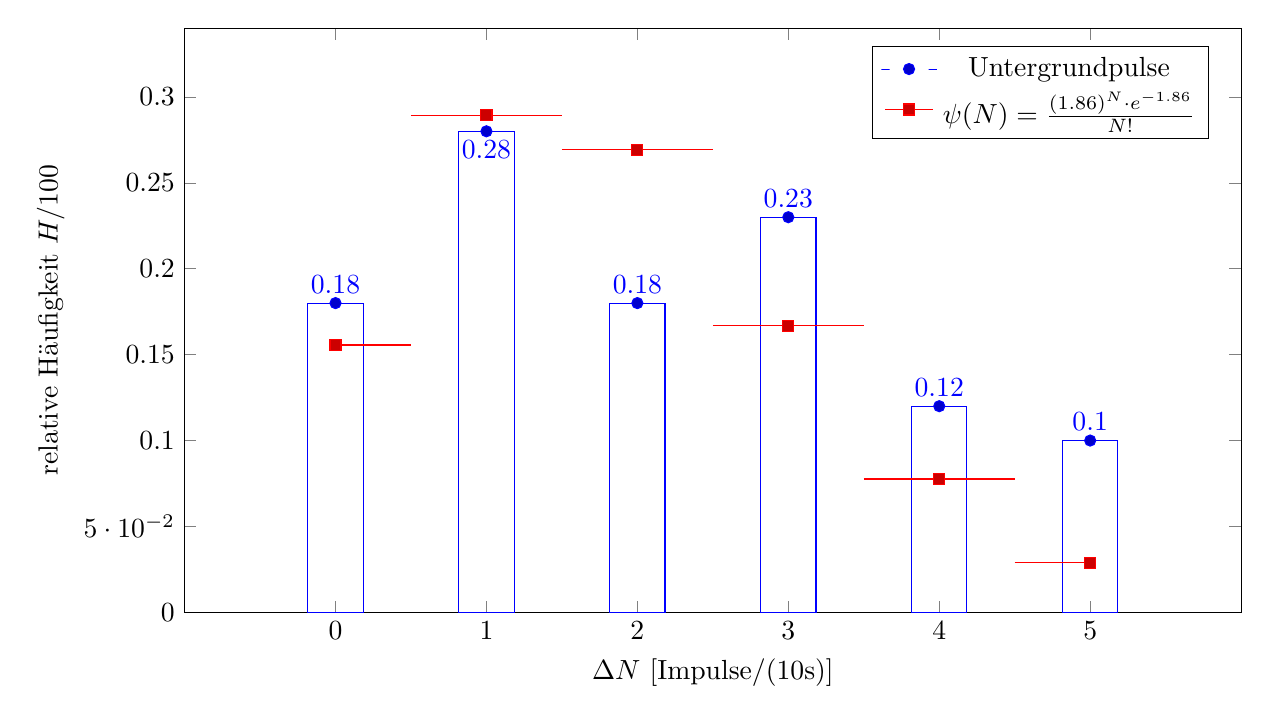
\begin{tikzpicture}
  \begin{axis}[
    width=15 cm,
    height=9 cm,
    xmin=-1, xmax=6,
    ymin=0, ymax=0.34,
    xlabel={$\Delta N$ [Impulse/(\SI{10}{s})]},
    ylabel={relative Häufigkeit $H/100$},
    domain=0:5,
		samples=6,
    legend entries={Untergrundpulse, $\psi(N)=\frac{(\num{1.86})^N\cdot e^{-\num{1.86}}}{N!}$},
    legend pos=north east,
		bar width=20pt,
		xtick={0,1,...,5}
  ]
  \addplot+[ybar, nodes near coords, forget plot] plot coordinates {
		(0,0.18)	(2,0.18)	(3,0.23)	(4,0.12)	(5,0.1)
		};
	\addplot+[ybar, nodes near coords, every node near coord/.append style={anchor=north}] plot coordinates {
		(1,0.28)
		};
	\addplot+[jump mark mid] {(1.86)^x*e^(-1.86)/factorial(x)};
  \end{axis}
\end{tikzpicture}
\caption{Relative Häufigkeitsverteilung der Untergrundpulse. Impulse innerhalb eines Intervalls von $\SI{10}{s}$ wurden zusammengefasst und die erwartete Poisson-Verteilung ist eingezeichnet}
\label{fig:untergrundrelativ}
\end{figure}

Die Quellen wurden gegen die Wand gerichtet und 100 mal die Zahl der Untergrundpulse in 10 Sekunden gemessen. Der Mittelwert für die Zahl der Pulse in 10 Sekunden beträgt $\bar{N}=\num{1.86}$ und die empirische Standardabweichung $\sigma_N=\num{1.34}$. Die absoluten bzw. relativen Häufigkeiten sind in den Diagrammen zu sehen. Zusätzlich wurde in \cref{fig:untergrundrelativ} die aus der Theorie erwartete Poisson-Verteilung eingezeichnet:
\begin{equation}
		\psi(N)=\frac{\bar{N}^N\cdot e^{-\bar{N}}}{N!}
		\label{eq:poisson}
	\end{equation}
	
	Diese stimmt mit den Messwerten insofern überein, als dass eine anfängliche Zunahme bis zum maximalen Wert für $\Delta N=1$ und eine anschließende Abnahme auf den minimalen Wert $\Delta N=5$  zu sehen ist. Allerdings fällt der Messwert für $\Delta N=2$ aus der Reihe.